\documentclass{standalone}
\usepackage{tikz}
\usetikzlibrary{patterns, positioning}


\begin{document}
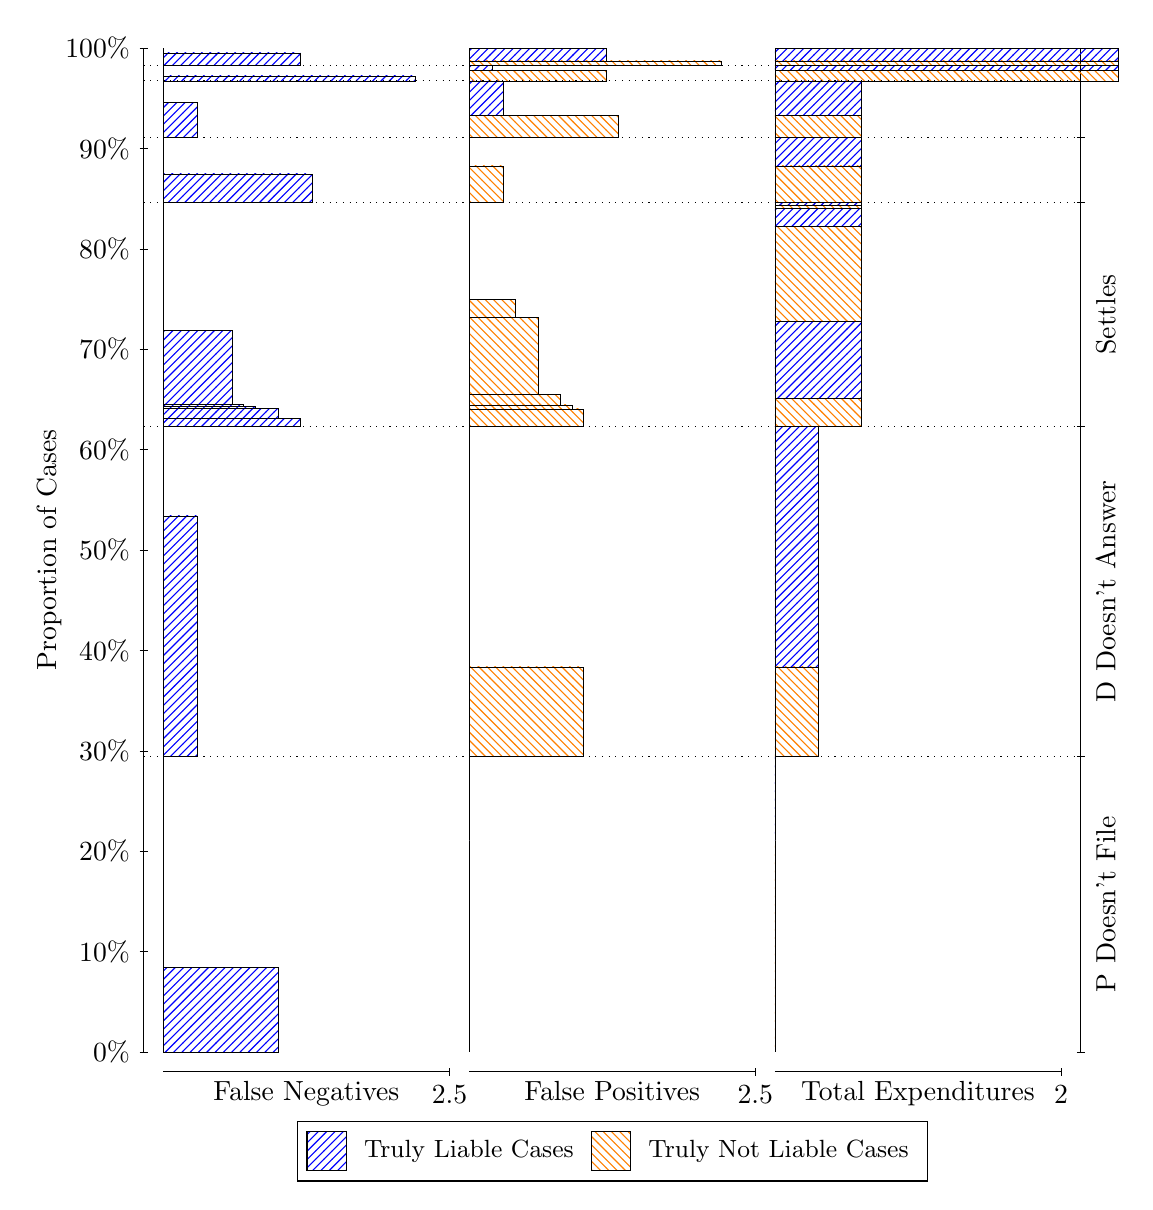
\begin{tikzpicture}
\draw[black, very thin] (1.5,1.75) -- (1.5,14.5);
\node[rotate=90, text=black, anchor=center] at (0.3, 8.125) {Proportion of Cases};
\draw[black, very thin] (1.45,1.75) -- (1.55,1.75);
\node[text=black, anchor=east] at (1.45, 1.75) {0\%};
\draw[black, very thin] (1.45,3.025) -- (1.55,3.025);
\node[text=black, anchor=east] at (1.45, 3.025) {10\%};
\draw[black, very thin] (1.45,4.3) -- (1.55,4.3);
\node[text=black, anchor=east] at (1.45, 4.3) {20\%};
\draw[black, very thin] (1.45,5.575) -- (1.55,5.575);
\node[text=black, anchor=east] at (1.45, 5.575) {30\%};
\draw[black, very thin] (1.45,6.85) -- (1.55,6.85);
\node[text=black, anchor=east] at (1.45, 6.85) {40\%};
\draw[black, very thin] (1.45,8.125) -- (1.55,8.125);
\node[text=black, anchor=east] at (1.45, 8.125) {50\%};
\draw[black, very thin] (1.45,9.4) -- (1.55,9.4);
\node[text=black, anchor=east] at (1.45, 9.4) {60\%};
\draw[black, very thin] (1.45,10.675) -- (1.55,10.675);
\node[text=black, anchor=east] at (1.45, 10.675) {70\%};
\draw[black, very thin] (1.45,11.95) -- (1.55,11.95);
\node[text=black, anchor=east] at (1.45, 11.95) {80\%};
\draw[black, very thin] (1.45,13.225) -- (1.55,13.225);
\node[text=black, anchor=east] at (1.45, 13.225) {90\%};
\draw[black, very thin] (1.45,14.5) -- (1.55,14.5);
\node[text=black, anchor=east] at (1.45, 14.5) {100\%};

\draw[black, very thin] (13.4,1.75) -- (13.4,14.5);
\draw[black, very thin] (13.35,1.75) -- (13.45,1.75);
\node[anchor=west] at (13.35, 1.75) {};
\draw[black, very thin] (13.35,5.5052) -- (13.45,5.5052);
\node[anchor=west] at (13.35, 5.5052) {};
\draw[black, very thin] (13.35,9.6951) -- (13.45,9.6951);
\node[anchor=west] at (13.35, 9.6951) {};
\draw[black, very thin] (13.35,12.536) -- (13.45,12.536);
\node[anchor=west] at (13.35, 12.536) {};
\draw[black, very thin] (13.35,13.368) -- (13.45,13.368);
\node[anchor=west] at (13.35, 13.368) {};
\draw[black, very thin] (13.35,14.084) -- (13.45,14.084);
\node[anchor=west] at (13.35, 14.084) {};
\draw[black, very thin] (13.35,14.275) -- (13.45,14.275);
\node[anchor=west] at (13.35, 14.275) {};
\draw[black, very thin] (13.35,14.5) -- (13.45,14.5);
\node[anchor=west] at (13.35, 14.5) {};

\draw[black, very thin, pattern color=blue, pattern=north east lines] (1.75,1.75) rectangle (3.2033,2.8196);
\draw[black, very thin, pattern color=orange, pattern=north west lines] (1.75,2.8196) rectangle (1.75,5.5052);
\draw[black, very thin, pattern color=blue, pattern=north east lines] (1.75,5.5052) rectangle (2.186,8.5596);
\draw[black, very thin, pattern color=orange, pattern=north west lines] (1.75,8.5596) rectangle (1.75,9.6951);
\draw[black, very thin, pattern color=blue, pattern=north east lines] (1.75,9.6951) rectangle (3.494,9.7924);
\draw[black, very thin, pattern color=blue, pattern=north east lines] (1.75,9.7924) rectangle (3.2033,9.9194);
\draw[black, very thin, pattern color=blue, pattern=north east lines] (1.75,9.9194) rectangle (2.9127,9.9516);
\draw[black, very thin, pattern color=blue, pattern=north east lines] (1.75,9.9516) rectangle (2.7673,9.9785);
\draw[black, very thin, pattern color=blue, pattern=north east lines] (1.75,9.9785) rectangle (2.622,10.918);
\draw[black, very thin, pattern color=orange, pattern=north west lines] (1.75,10.918) rectangle (1.75,12.536);
\draw[black, very thin, pattern color=blue, pattern=north east lines] (1.75,12.536) rectangle (3.6393,12.901);
\draw[black, very thin, pattern color=orange, pattern=north west lines] (1.75,12.901) rectangle (1.75,13.368);
\draw[black, very thin, pattern color=blue, pattern=north east lines] (1.75,13.368) rectangle (2.186,13.806);
\draw[black, very thin, pattern color=orange, pattern=north west lines] (1.75,13.806) rectangle (1.75,14.084);
\draw[black, very thin, pattern color=blue, pattern=north east lines] (1.75,14.084) rectangle (4.9473,14.145);
\draw[black, very thin, pattern color=orange, pattern=north west lines] (1.75,14.145) rectangle (1.75,14.275);
\draw[black, very thin, pattern color=blue, pattern=north east lines] (1.75,14.275) rectangle (3.494,14.438);
\draw[black, very thin, pattern color=orange, pattern=north west lines] (1.75,14.438) rectangle (1.75,14.5);
\draw[black, very thin, pattern color=orange, pattern=north west lines] (5.6333,1.75) rectangle (5.6333,4.4355);
\draw[black, very thin, pattern color=blue, pattern=north east lines] (5.6333,4.4355) rectangle (5.6333,5.5052);
\draw[black, very thin, pattern color=orange, pattern=north west lines] (5.6333,5.5052) rectangle (7.0867,6.6408);
\draw[black, very thin, pattern color=blue, pattern=north east lines] (5.6333,6.6408) rectangle (5.6333,9.6951);
\draw[black, very thin, pattern color=orange, pattern=north west lines] (5.6333,9.6951) rectangle (7.0867,9.9184);
\draw[black, very thin, pattern color=orange, pattern=north west lines] (5.6333,9.9184) rectangle (6.9413,9.9669);
\draw[black, very thin, pattern color=orange, pattern=north west lines] (5.6333,9.9669) rectangle (6.796,10.101);
\draw[black, very thin, pattern color=orange, pattern=north west lines] (5.6333,10.101) rectangle (6.5053,11.079);
\draw[black, very thin, pattern color=orange, pattern=north west lines] (5.6333,11.079) rectangle (6.2147,11.312);
\draw[black, very thin, pattern color=blue, pattern=north east lines] (5.6333,11.312) rectangle (5.6333,12.536);
\draw[black, very thin, pattern color=orange, pattern=north west lines] (5.6333,12.536) rectangle (6.0693,13.003);
\draw[black, very thin, pattern color=blue, pattern=north east lines] (5.6333,13.003) rectangle (5.6333,13.368);
\draw[black, very thin, pattern color=orange, pattern=north west lines] (5.6333,13.368) rectangle (7.5227,13.646);
\draw[black, very thin, pattern color=blue, pattern=north east lines] (5.6333,13.646) rectangle (6.0693,14.084);
\draw[black, very thin, pattern color=orange, pattern=north west lines] (5.6333,14.084) rectangle (7.3773,14.214);
\draw[black, very thin, pattern color=blue, pattern=north east lines] (5.6333,14.214) rectangle (5.924,14.275);
\draw[black, very thin, pattern color=orange, pattern=north west lines] (5.6333,14.275) rectangle (8.8307,14.337);
\draw[black, very thin, pattern color=blue, pattern=north east lines] (5.6333,14.337) rectangle (7.3773,14.5);
\draw[black, very thin, pattern color=orange, pattern=north west lines] (9.5167,1.75) rectangle (9.5167,4.4355);
\draw[black, very thin, pattern color=blue, pattern=north east lines] (9.5167,4.4355) rectangle (9.5167,5.5052);
\draw[black, very thin, pattern color=orange, pattern=north west lines] (9.5167,5.5052) rectangle (10.062,6.6408);
\draw[black, very thin, pattern color=blue, pattern=north east lines] (9.5167,6.6408) rectangle (10.062,9.6951);
\draw[black, very thin, pattern color=orange, pattern=north west lines] (9.5167,9.6951) rectangle (10.607,10.052);
\draw[black, very thin, pattern color=blue, pattern=north east lines] (9.5167,10.052) rectangle (10.607,11.024);
\draw[black, very thin, pattern color=orange, pattern=north west lines] (9.5167,11.024) rectangle (10.607,12.236);
\draw[black, very thin, pattern color=blue, pattern=north east lines] (9.5167,12.236) rectangle (10.607,12.46);
\draw[black, very thin, pattern color=orange, pattern=north west lines] (9.5167,12.46) rectangle (10.607,12.509);
\draw[black, very thin, pattern color=blue, pattern=north east lines] (9.5167,12.509) rectangle (10.607,12.536);
\draw[black, very thin, pattern color=orange, pattern=north west lines] (9.5167,12.536) rectangle (10.607,13.003);
\draw[black, very thin, pattern color=blue, pattern=north east lines] (9.5167,13.003) rectangle (10.607,13.368);
\draw[black, very thin, pattern color=orange, pattern=north west lines] (9.5167,13.368) rectangle (10.607,13.646);
\draw[black, very thin, pattern color=blue, pattern=north east lines] (9.5167,13.646) rectangle (10.607,14.084);
\draw[black, very thin, pattern color=orange, pattern=north west lines] (9.5167,14.084) rectangle (13.877,14.214);
\draw[black, very thin, pattern color=blue, pattern=north east lines] (9.5167,14.214) rectangle (13.877,14.275);
\draw[black, very thin, pattern color=orange, pattern=north west lines] (9.5167,14.275) rectangle (13.877,14.337);
\draw[black, very thin, pattern color=blue, pattern=north east lines] (9.5167,14.337) rectangle (13.877,14.5);
\draw[black, dotted] (1.5,5.5052) -- (13.4,5.5052);
\draw[black, dotted] (1.5,9.6951) -- (13.4,9.6951);
\draw[black, dotted] (1.5,12.536) -- (13.4,12.536);
\draw[black, dotted] (1.5,13.368) -- (13.4,13.368);
\draw[black, dotted] (1.5,14.084) -- (13.4,14.084);
\draw[black, dotted] (1.5,14.275) -- (13.4,14.275);
\draw[black, very thin] (1.75,1.5) -- (5.3833,1.5);
\node[text=black, anchor=north] at (3.5667, 1.5) {False Negatives};
\draw[black, very thin] (5.3833,1.45) -- (5.3833,1.55);
\node[text=black, anchor=north] at (5.3833, 1.45) {2.5};

\draw[black, very thin] (5.6333,1.5) -- (9.2667,1.5);
\node[text=black, anchor=north] at (7.45, 1.5) {False Positives};
\draw[black, very thin] (9.2667,1.45) -- (9.2667,1.55);
\node[text=black, anchor=north] at (9.2667, 1.45) {2.5};

\draw[black, very thin] (9.5167,1.5) -- (13.15,1.5);
\node[text=black, anchor=north] at (11.333, 1.5) {Total Expenditures};
\draw[black, very thin] (13.15,1.45) -- (13.15,1.55);
\node[text=black, anchor=north] at (13.15, 1.45) {2};

\node[text=black, centered, rotate=90] at (13.72, 3.6276) {P Doesn't File};
\node[text=black, centered, rotate=90] at (13.72, 7.6002) {D Doesn't Answer};
\node[text=black, centered, rotate=90] at (13.72, 11.115) {Settles};





\draw (7.449999999999999,1.5) node[draw=none] (baseCoordinate) {};
\begin{scope}[align=center]
        \matrix[scale=0.5, draw=black, below=0.5cm of baseCoordinate, nodes={draw}, column sep=0.1cm]{
            \node[rectangle, draw, minimum width=0.5cm, minimum height=0.5cm, pattern color=blue, pattern=north east lines] {}; &
            \node[draw=none, font=\small, text=black] (B) {Truly Liable Cases}; &
            \node[rectangle, draw, minimum width=0.5cm, minimum height=0.5cm, pattern color=orange, pattern=north west lines] {}; &
            \node[draw=none, font=\small, text=black] (B) {Truly Not Liable Cases}; \\
            };
\end{scope}

\end{tikzpicture}
\end{document}